\documentclass[12pt,a4paper]{ctexart}

\usepackage[a4paper,margin=2.2cm]{geometry}
\usepackage{graphicx}
\usepackage{float}
\usepackage{booktabs}
\usepackage{siunitx}
\usepackage{hyperref}
\usepackage{caption}
\usepackage{amsmath}
\usepackage{subcaption}
\usepackage{xcolor}
\usepackage{listings}

\hypersetup{colorlinks=true,linkcolor=black,urlcolor=blue,citecolor=black}
\captionsetup{font=small,labelfont=bf}
\lstset{
    language=Matlab,
    basicstyle=\ttfamily\small,
    keywordstyle=\color{blue!70!black},
    commentstyle=\color{green!40!black},
    stringstyle=\color{orange!60!black},
    numbers=left,
    numberstyle=\scriptsize\color{gray},
    stepnumber=1,
    numbersep=6pt,
    frame=single,
    breaklines=true,
    showstringspaces=false
}

\title{\vspace{-1.2cm}EE328 语音信号处理实验五\\}

\author{
    12313505 胡伟毅\and
    12310403 安文博
}
\date{\today}

\begin{document}
\maketitle
\thispagestyle{empty}

\section{引言}
本次实验围绕短时频域分析（Short-Time Spectral Analysis, STSA）展开，核心目标是通过“分帧—加窗—频谱计算”的流程，观察语音信号在时间与频率两域中的局部结构。与仅看整段频谱相比，短时分析能够更清楚地反映非平稳语音在不同时间片段的频率组成变化。

本报告分为三个问题：Problem 1 聚焦单帧分析，验证窗函数与零填充对谱线可读性的作用；Problem 2 比较多种窗长和两类窗函数（Hamming/Rectangular）对短时谱估计的影响；Problem 3 基于语谱图进行连续短时分析，讨论重采样、窗长、FFT 长度、幅度尺度与颜色映射等参数对时频图显示效果的影响。

\section{实验内容与结果分析}

\subsection{Problem 1：单帧短时谱分析}
\subsubsection*{题目要求}
实现函数 \texttt{STSA\_SingleFrame(filename, startsmp, framelength)}，输入语音文件、起始采样点和帧长（ms），完成以下四项绘图：
\begin{enumerate}
    \item 整段语音波形；
    \item 指定起点处的加窗帧波形；
    \item 该帧 STFT 幅度谱；
    \item 该帧 STFT 对数幅度谱（dB）。
\end{enumerate}
并使用课件给定测试参数：\texttt{s5.wav}（\texttt{startsmp=7000}）与 \texttt{vowel\_iy\_100hz.wav}（\texttt{startsmp=1000}），帧长均为 \SI{40}{ms}。

\subsubsection*{实现方法}
设采样率为 $F_s$，输入帧长为 $T_{\text{ms}}$（单位 ms），则样本点数为
\begin{equation}
L = \mathrm{round}(T_{\text{ms}}\cdot 10^{-3}F_s).
\end{equation}
在起始点 $n_0$ 处截取单帧 $x_f[m]$，乘以 Hamming 窗 $w[m]$ 得到
\begin{equation}
\tilde{x}_f[m] = x_f[m]w[m],\quad 0\le m\le L-1.
\end{equation}
随后进行零填充 FFT（本实现中取不小于 $4L$ 的 2 次幂）以提升频域采样密度，得到
\begin{equation}
X[k] = \sum_{m=0}^{L-1}\tilde{x}_f[m]e^{-j2\pi km/N_{\text{FFT}}},
\end{equation}
并分别绘制 $|X[k]|$ 与 $20\log_{10}(|X[k]|+\varepsilon)$。

\subsubsection*{关键代码段}
\begin{lstlisting}[caption={Problem 1：单帧 STFT 与对数幅度谱}]
frameLenSamples = round(framelength * 1e-3 * fs);
frame = zeros(frameLenSamples, 1);
endIdx = min(startsmp + frameLenSamples - 1, numel(x));
frame(1:endIdx-startsmp+1) = x(startsmp:endIdx);

w = hamming(frameLenSamples);
xw = frame .* w;
nfft = 2^nextpow2(max(512, 4 * frameLenSamples));
X = fft(xw, nfft);
mag = abs(X(1:nfft/2+1));
magdB = 20 * log10(mag + eps);
\end{lstlisting}

\begin{figure}[H]
    \centering
    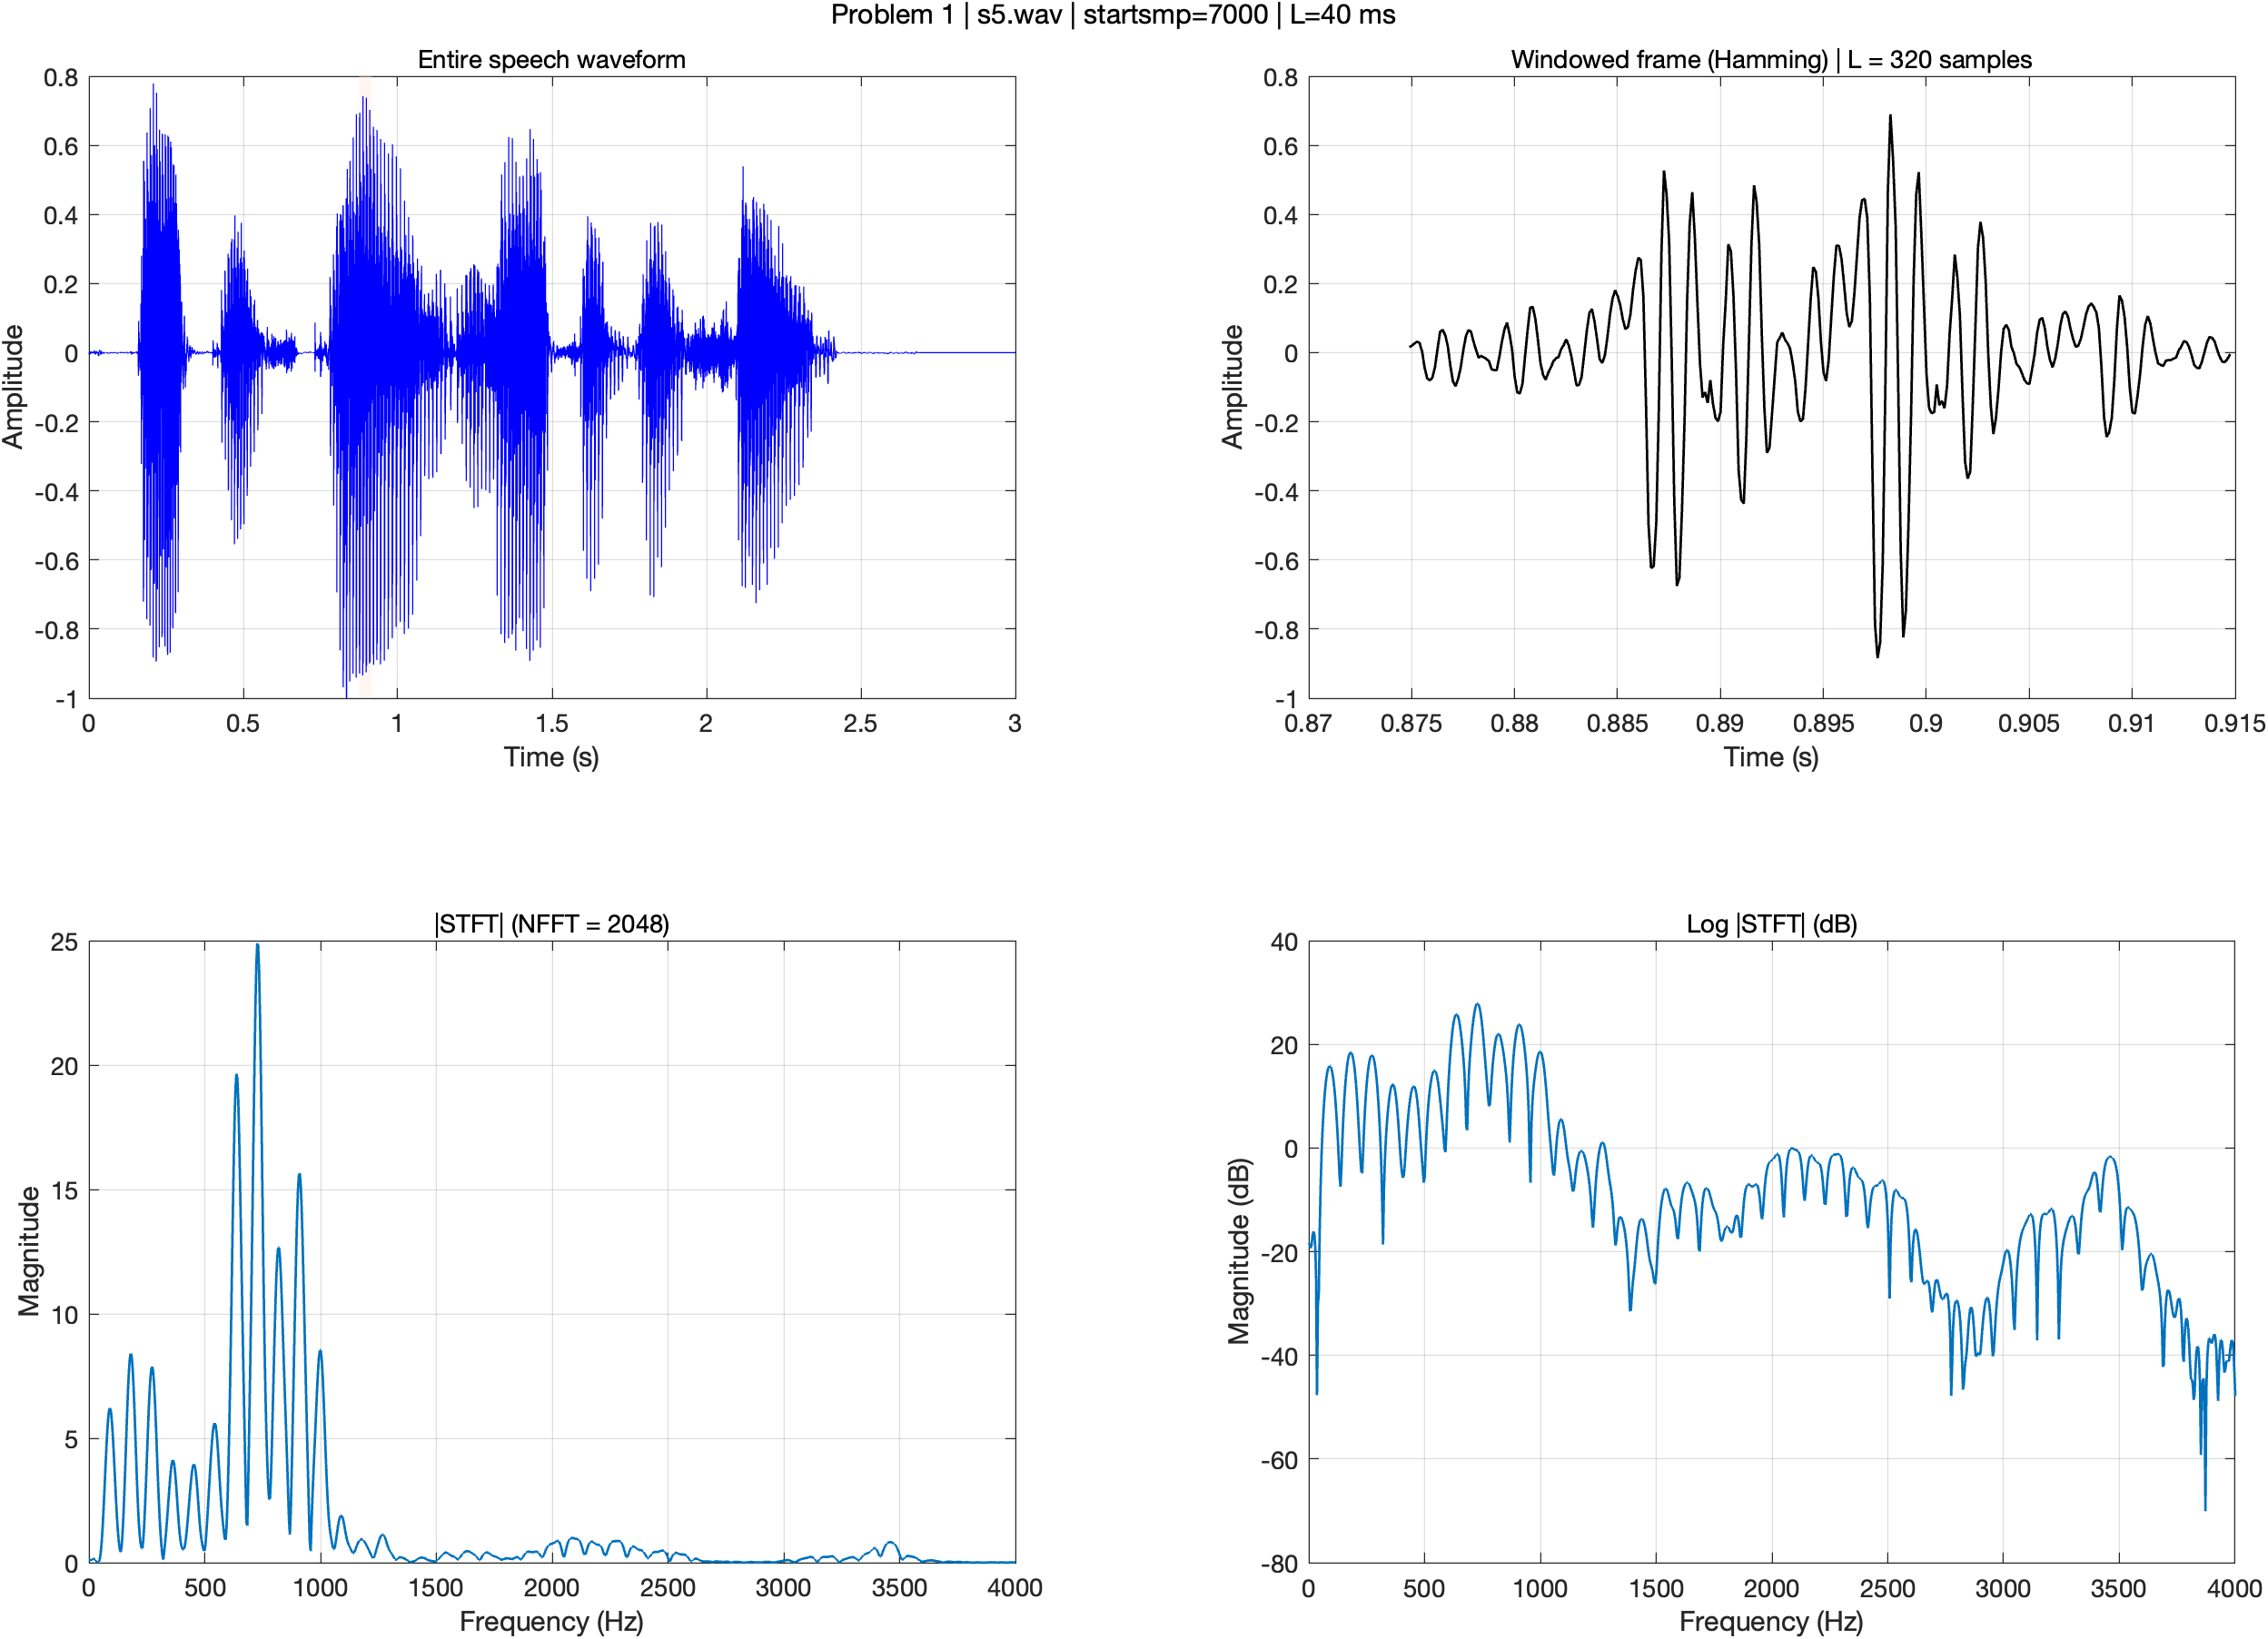
\includegraphics[width=0.95\textwidth]{figures/p1_s5_start7000_L40ms.png}
    \caption{Problem 1 结果（\texttt{s5.wav}, \texttt{startsmp=7000}, \texttt{L=40 ms}）}
    \label{fig:p1_s5}
\end{figure}

\begin{figure}[H]
    \centering
    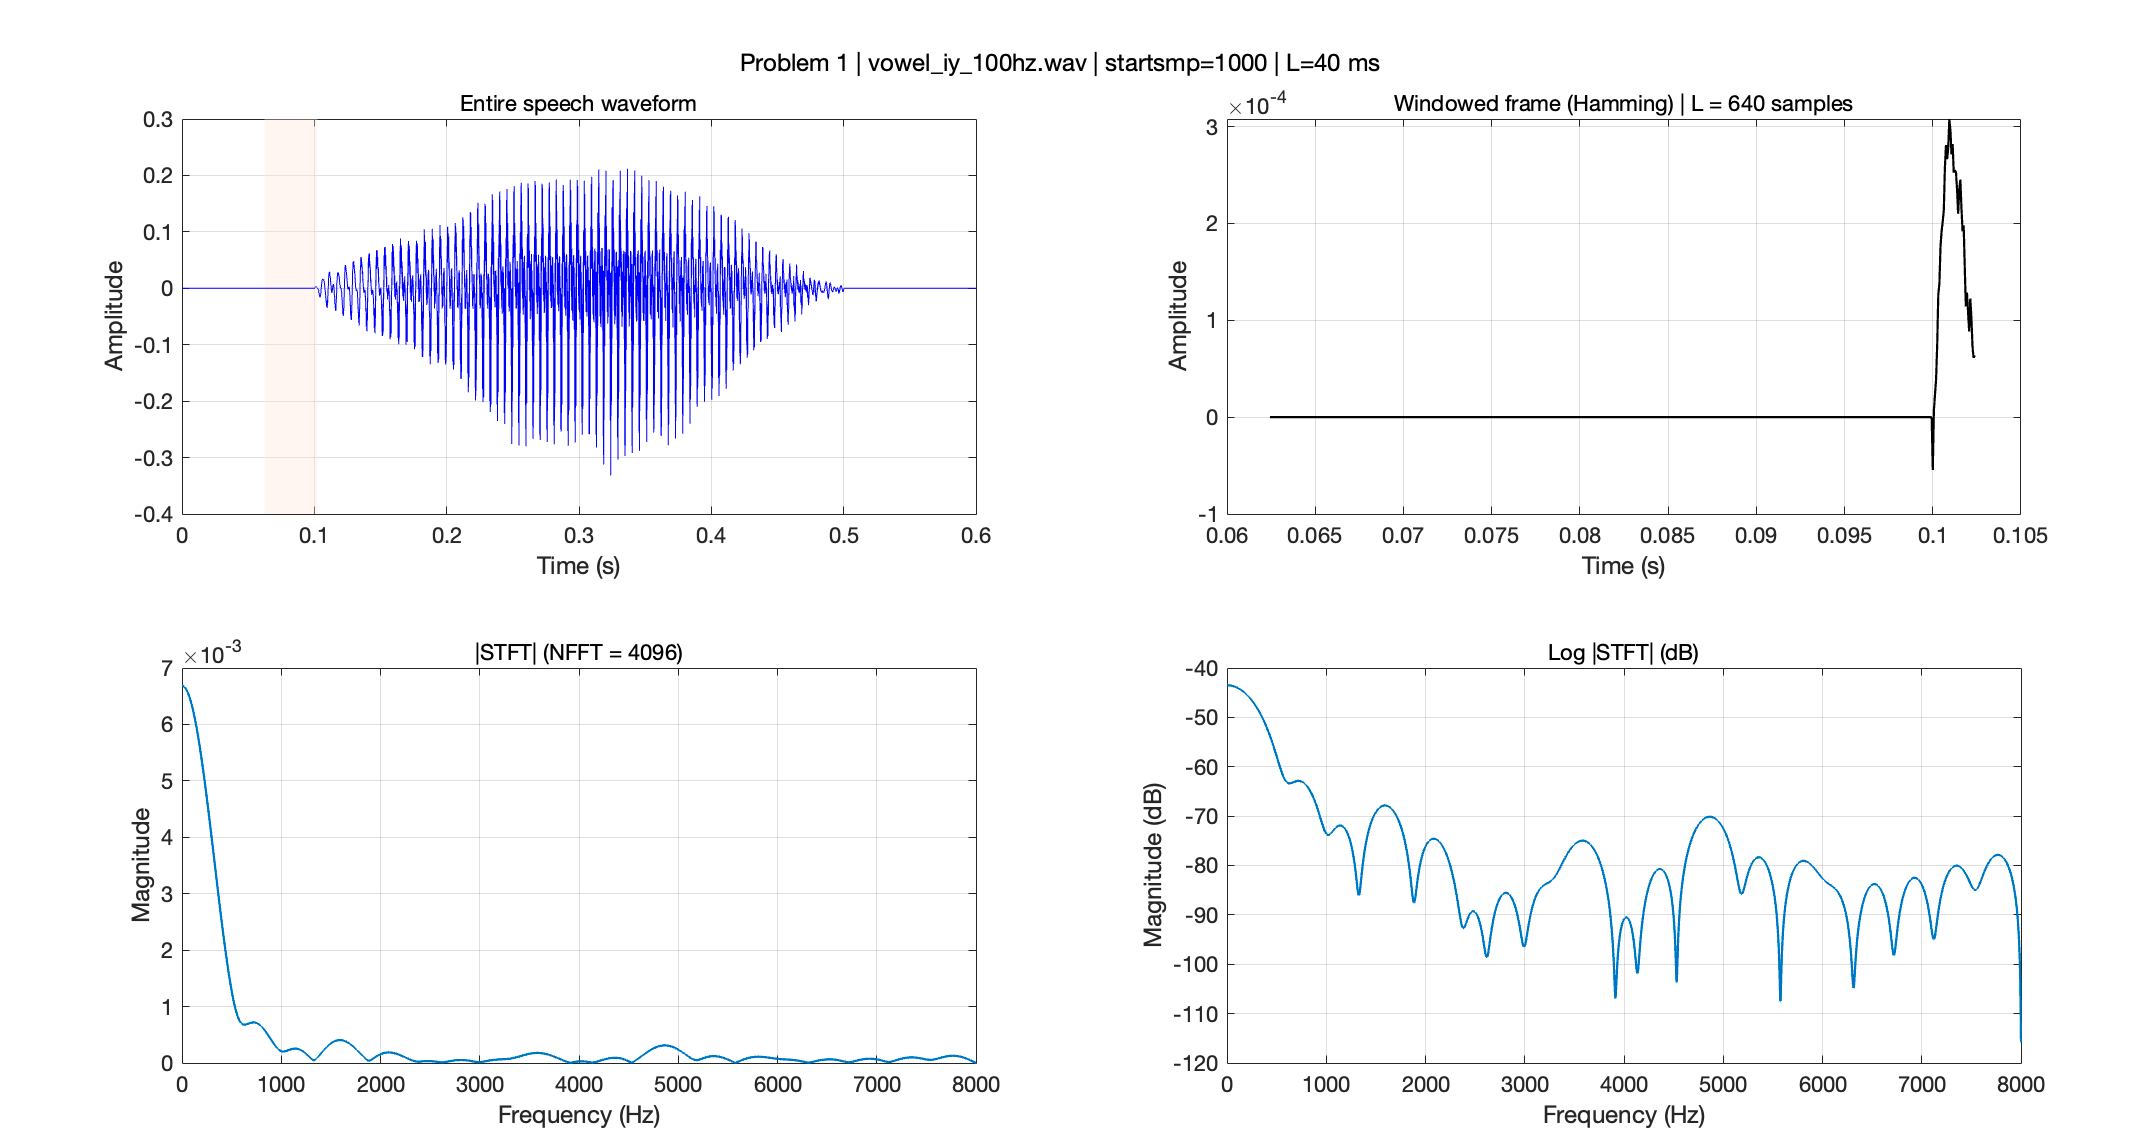
\includegraphics[width=0.95\textwidth]{figures/p1_test.png}
    \caption{Problem 1 结果（\texttt{vowel\_iy\_100hz.wav}, \texttt{startsmp=1000}, \texttt{L=40 ms}）}
    \label{fig:p1_vowel}
\end{figure}

\subsubsection*{结果与回答}
图~\ref{fig:p1_s5} 与图~\ref{fig:p1_vowel} 反映了两类不同片段的单帧频谱特征。对于 \texttt{s5.wav}（起点 7000），所选帧位于明显有声段，窗后波形仍具有较强周期性；在线性幅度谱中，低频到中频段出现多个峰值，说明该帧包含较丰富的谐波结构。对应的对数谱进一步拉开了强弱分量对比，弱峰与谱谷更容易分辨，这有助于观察共振峰附近的能量起伏。

对于 \texttt{vowel\_iy\_100hz.wav}（起点 1000），该帧整体幅度更小，窗后波形在时域上能量集中但有效振动时间较短，线性谱中主要能量集中在较低频带，较高频段能量快速衰减。对数谱中可见主峰之外的频率分量整体处于较低电平区间，符合元音片段在该取样位置下“主共振峰明显、背景分量较弱”的典型表现。

从算法角度看，本题还有两点可验证的现象。第一，Hamming 窗削弱了截断处突变，谱曲线相较于裸截帧更平滑，旁瓣泄漏更可控；第二，零填充使频率采样更密，曲线显示更连续，便于读图，但不会改变物理意义上的真实分辨率。综上，我们完成了“单帧时域—频域”对应关系的直观验证。

\subsection{Problem 2：多窗长与窗型比较}
\subsubsection*{题目要求}
实现函数 \texttt{STSA\_MultiLengths(num, filename, startsmp, framelengths)}，比较多种窗长下的短时谱结果。除窗长比较外，还需分别使用 Hamming 与 Rectangular 两种窗型。课件建议测试：\texttt{s5.wav}、\texttt{num=4}、\texttt{framelengths=[5,10,20,40] ms}、\texttt{startsmp=7000}。

\subsubsection*{实现方法}
对每个窗长 $L_i$，重复执行“截帧—加窗—FFT—绘图”流程，并在同一坐标系叠加不同窗长曲线（不同颜色）。每种窗型输出一张四子图页面，包括：
\begin{enumerate}
    \item 整段语音波形；
    \item 不同窗长对应的窗后帧波形叠加；
    \item 线性幅度谱叠加；
    \item 对数幅度谱叠加。
\end{enumerate}

\subsubsection*{关键代码段}
\begin{lstlisting}[caption={Problem 2：多窗长 + 两种窗函数比较}]
frameLens = round(framelengths * 1e-3 * fs);
nfft = 2^nextpow2(max(512, 4 * max(frameLens)));

plotForWindowType("Hamming window", true);
plotForWindowType("Rectangular window", false);

for k = 1:num
    N = frameLens(k);
    frame = extractFrame(x, startsmp, N);
    w = hamming(N);
    if ~useHamming
        w = ones(N, 1);
    end
    X = fft(frame .* w, nfft);
    mag = abs(X(1:nfft/2+1));
    magdB = 20 * log10(mag + eps);
end
\end{lstlisting}

\begin{figure}[H]
    \centering
    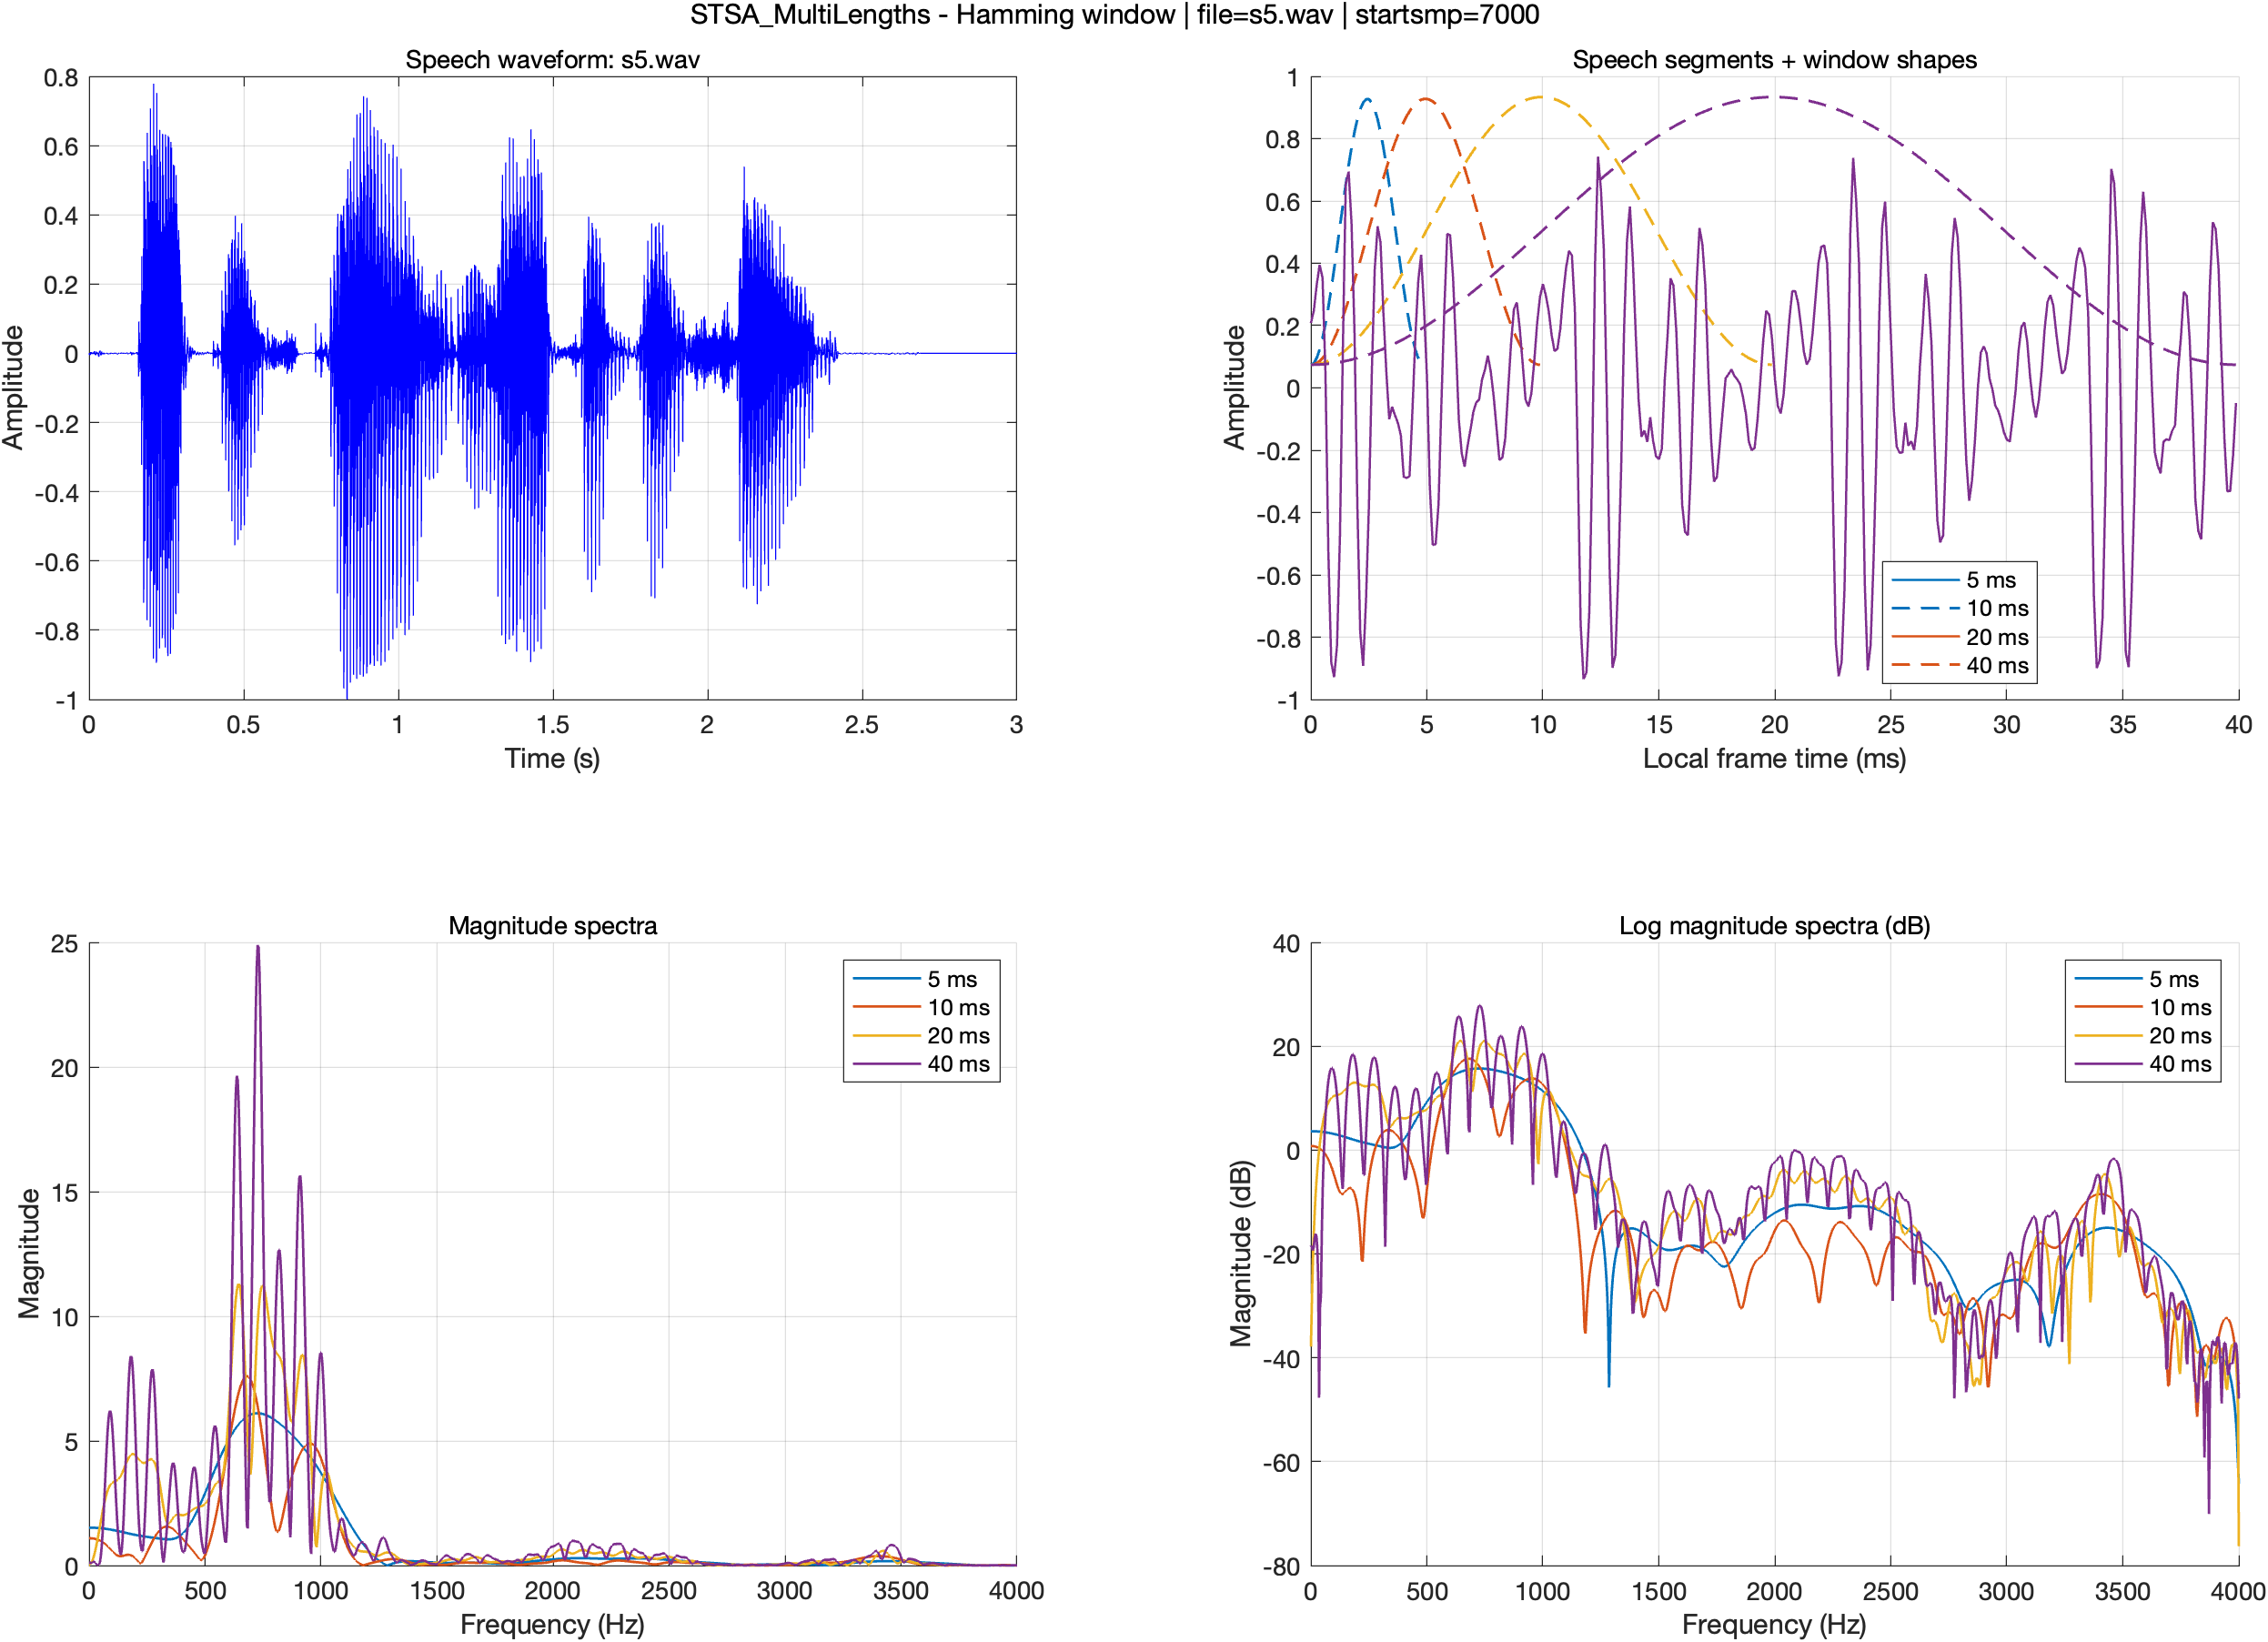
\includegraphics[width=0.95\textwidth]{figures/p2_s5_hammingwindow_start7000_L5_10_20_40.png}
    \caption{Problem 2 结果：Hamming 窗，多窗长比较}
    \label{fig:p2_hamming}
\end{figure}

\begin{figure}[H]
    \centering
    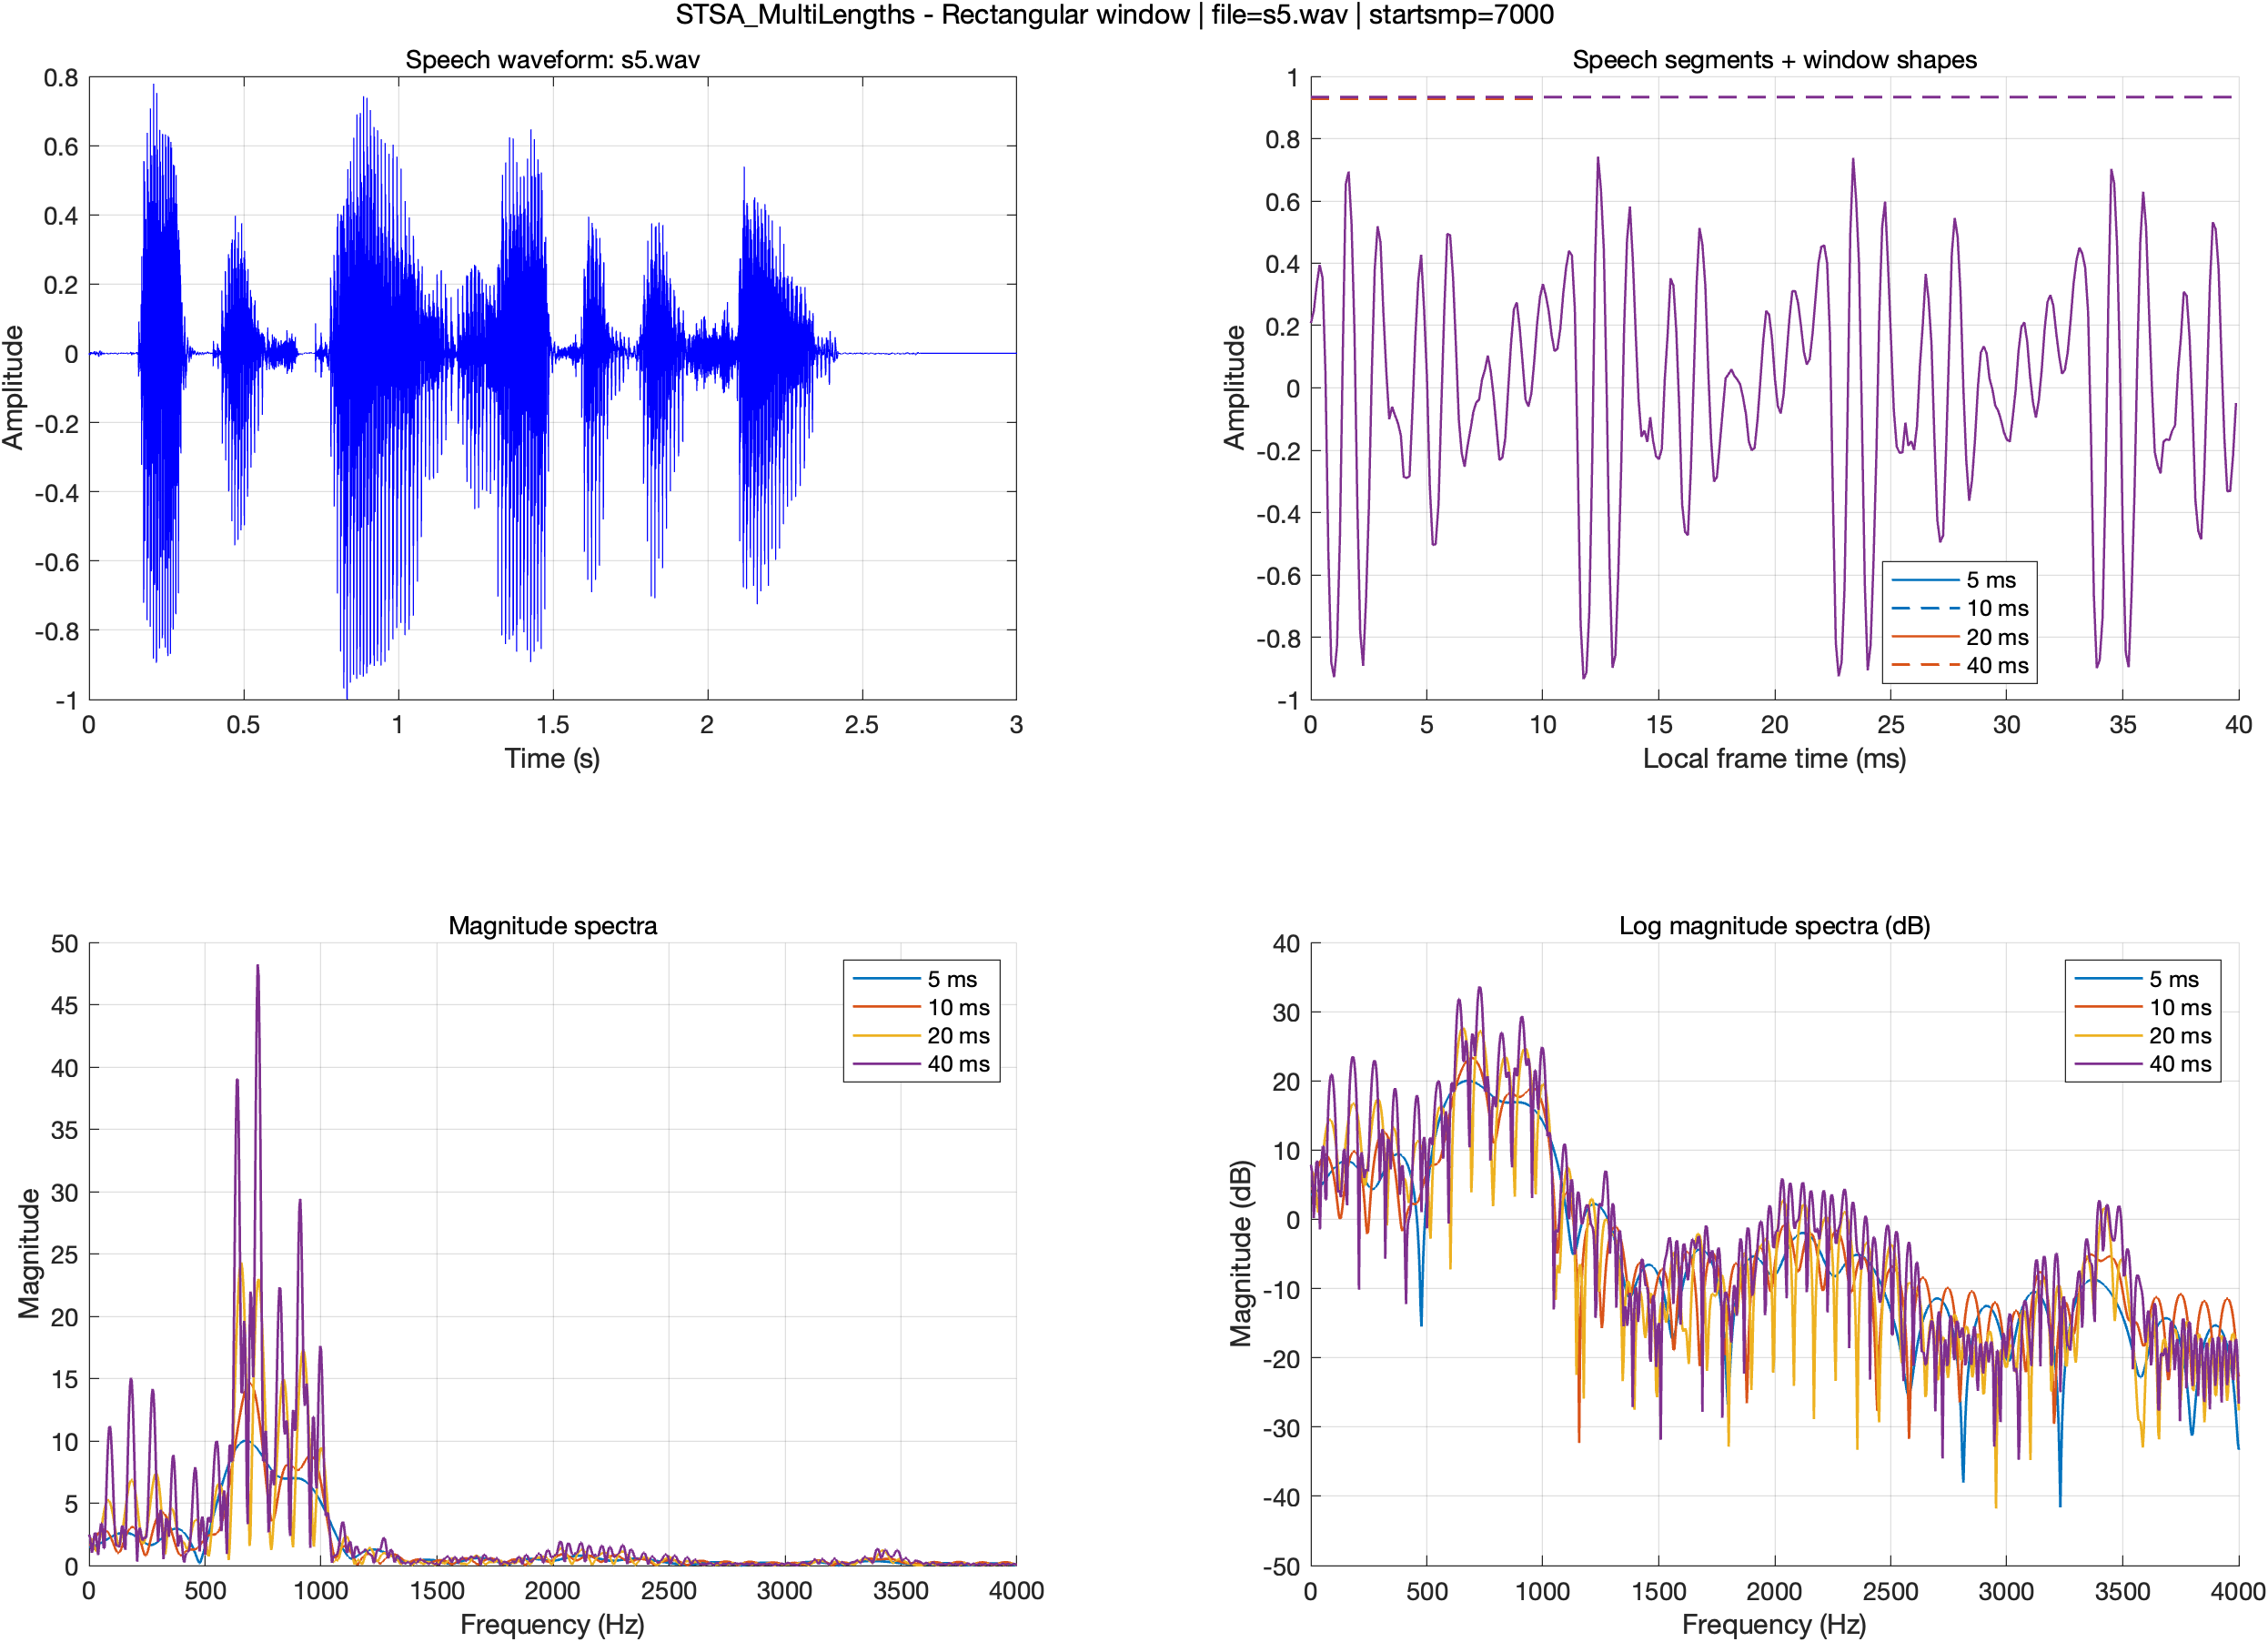
\includegraphics[width=0.95\textwidth]{figures/p2_s5_rectangularwindow_start7000_L5_10_20_40.png}
    \caption{Problem 2 结果：Rectangular 窗，多窗长比较}
    \label{fig:p2_rect}
\end{figure}

\subsubsection*{结果与回答}
从图~\ref{fig:p2_hamming} 与图~\ref{fig:p2_rect} 可观察到以下规律：
\begin{enumerate}
    \item 随窗长从 5 ms 增大到 40 ms，线性谱主瓣逐渐收窄、峰位更稳定，频率分辨率提升；但时间局部变化会被更强地平均，快速细节被弱化。
    \item 短窗（如 5 ms）对时域瞬时变化更敏感，能够保留更多快速波动信息，但频谱上主瓣更宽、曲线抖动更明显，细小峰值不易稳定分离。
    \item 在同一窗长下，矩形窗在对数谱中出现更多细碎波纹和较高的背景起伏，体现出更明显的旁瓣泄漏；Hamming 窗的对数谱更平滑，主峰周围结构更清晰。
\end{enumerate}

另外，从第二行“窗后时域片段”也能看出窗型差异：矩形窗等权截取，边缘突变更直接；Hamming 窗在帧边界处逐渐衰减，有助于减弱边界不连续性。结合第三、四行频谱图可知，窗长与窗型并非独立影响，它们共同决定了短时谱的可读性和稳定性。因此，Problem 2 的主要结论是：参数选择需要围绕任务目标做折中，若更关注频谱细节和噪声抑制，通常优先选择较平滑窗型并适当增大窗长；若更关注时间定位，则应采用更短分析窗。

\subsection{Problem 3：宽带/窄带语谱图}
\subsubsection*{题目要求}
实现函数 \texttt{STSA\_Spectrogram(filename, resamplerate, windowlengths, FFTlengths, magscale, range, color)}，在单页中绘制宽带与窄带语谱图，并支持如下参数：重采样选项、两种窗长、两种 FFT 长度、线性/对数幅度、动态范围、灰度或彩色显示。
此外，依据题目 bonus 要求，采用“手写 STFT”方式生成语谱图序列，而非直接调用内置 \texttt{spectrogram} 完成核心计算。

本次运行采用课件默认测试参数：
\begin{itemize}
    \item \texttt{filename = s5.wav}；
    \item \texttt{resamplerate = 0}（不重采样）；
    \item \texttt{windowlengths = [5, 50] ms}（宽带/窄带）；
    \item \texttt{FFTlengths = [1024, 1024]}；
    \item \texttt{magscale = log}；
    \item \texttt{range = 60 dB}；
    \item \texttt{color = color} 与 \texttt{gray} 各绘制一张。
\end{itemize}

\subsubsection*{实现方法}
短时谱定义为
\begin{equation}
X_n(e^{j\omega}) = \sum_m x[m]w[n-m]e^{-j\omega m}.
\end{equation}
将每帧频谱沿时间轴堆叠可得语谱图。实现中采用手写 STFT 流程：按 hop 长度滑动分帧、逐帧加窗、执行 FFT、截取单边频谱并拼接为时频矩阵。帧重叠率设置为 \(75\%\)，即
\begin{equation}
\texttt{noverlap}=0.75L.
\end{equation}
对数幅度下采用
\begin{equation}
S_{\mathrm{dB}} = 20\log_{10}(|S|+\varepsilon),
\end{equation}
并按 \texttt{range} 设置颜色轴显示范围。

\subsubsection*{关键代码段}
\begin{lstlisting}[caption={Problem 3（bonus）：手写 STFT 语谱图生成}]
if resamplerate > 0 && resamplerate ~= fs
    x = resample(x, resamplerate, fs);
    fs = resamplerate;
end

Lwide = round(windowlengths(1) * 1e-3 * fs);
Lnarrow = round(windowlengths(2) * 1e-3 * fs);
[Swide, fWide, tWide] = manualSTFT(x, fs, hamming(Lwide), FFTwide, round(0.75*Lwide));
[Snarrow, fNarrow, tNarrow] = manualSTFT(x, fs, hamming(Lnarrow), FFTnarrow, round(0.75*Lnarrow));

function [S, f, t] = manualSTFT(x, fs, w, nfft, noverlap)
    L = numel(w); hop = L - noverlap;
    numFrames = ceil((numel(x)-L)/hop) + 1;
    xPad = [x(:); zeros((numFrames-1)*hop + L - numel(x), 1)];
    kMax = floor(nfft/2); S = zeros(kMax+1, numFrames);
    for n = 1:numFrames
        idx0 = (n-1)*hop + 1;
        X = fft(xPad(idx0:idx0+L-1).*w, nfft);
        S(:, n) = X(1:kMax+1);
        t(n) = (idx0 - 1 + (L - 1)/2) / fs;
    end
    f = (0:kMax)' * fs / nfft;
end

Mwide = mag2db(abs(Swide) + eps);
Mnarrow = mag2db(abs(Snarrow) + eps);
imagesc(tWide, fWide, Mwide); set(gca, "YDir", "normal");
imagesc(tNarrow, fNarrow, Mnarrow); set(gca, "YDir", "normal");
\end{lstlisting}

\begin{figure}[H]
    \centering
    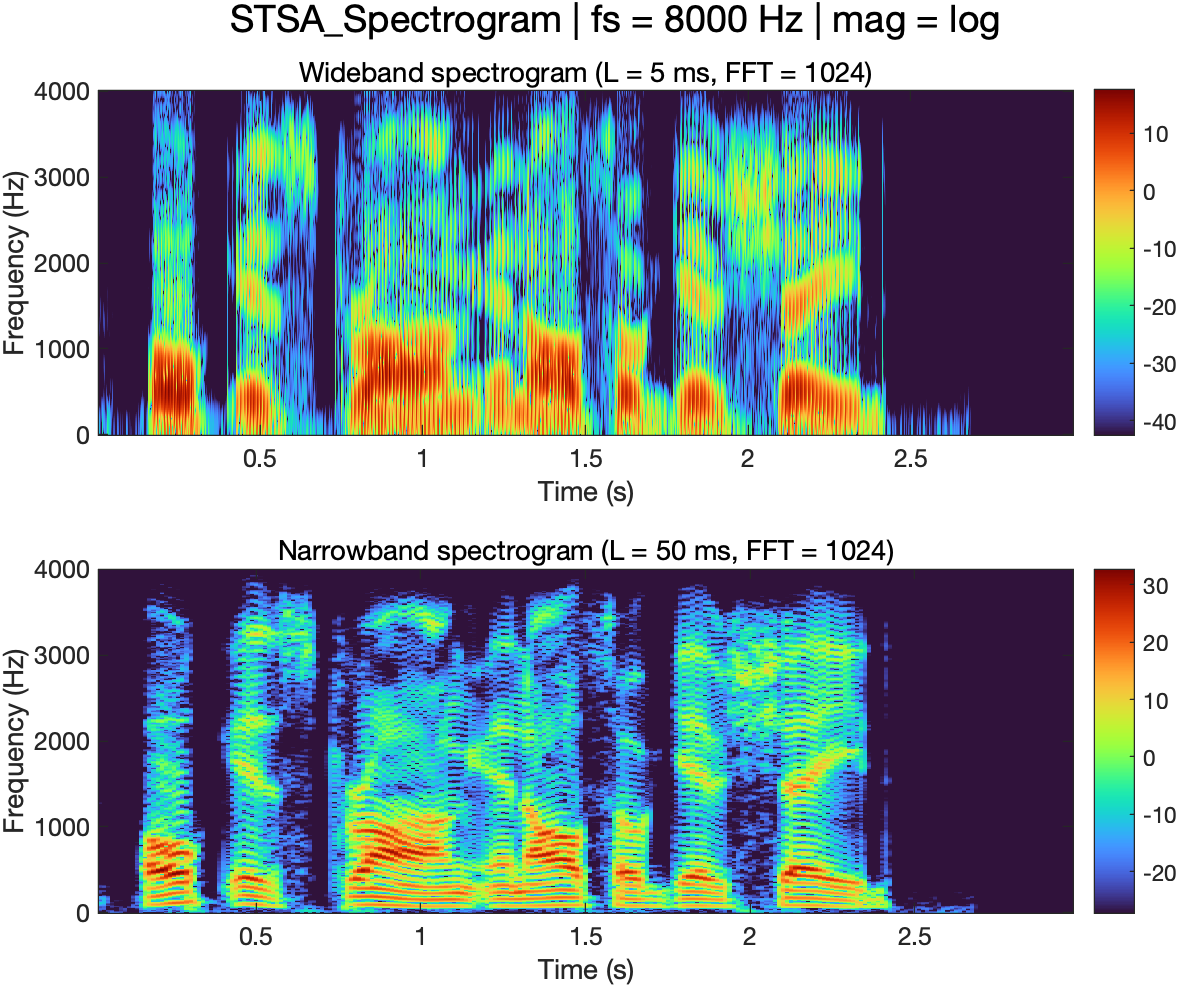
\includegraphics[width=0.85\textwidth]{figures/p3_s5_fs8000_win5_50_fft1024_1024_log_r60_color.png}
    \caption{Problem 3 结果：彩色语谱图（\texttt{log}, \texttt{range=60 dB}）}
    \label{fig:p3_color}
\end{figure}

\begin{figure}[H]
    \centering
    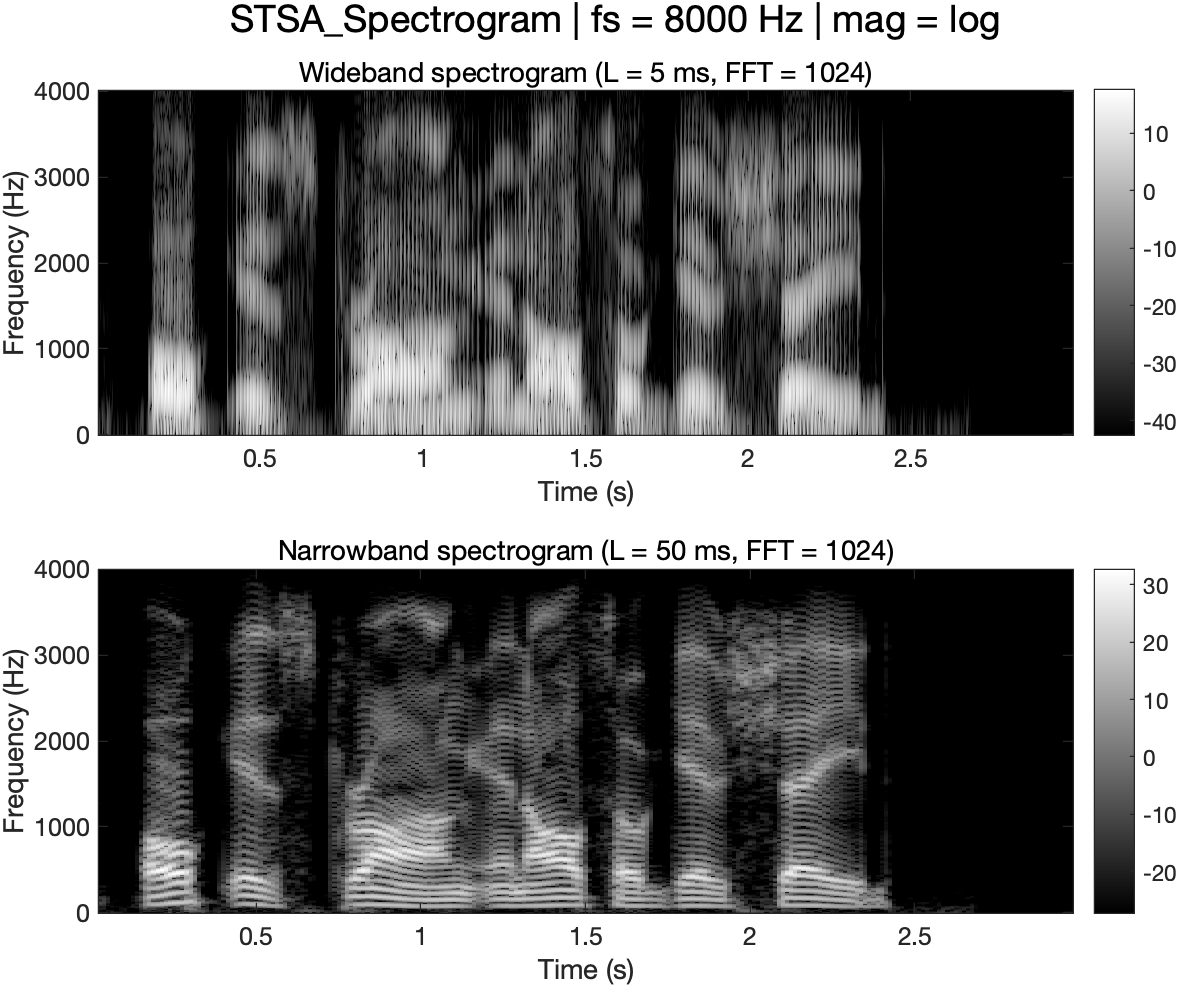
\includegraphics[width=0.85\textwidth]{figures/p3_s5_fs8000_win5_50_fft1024_1024_log_r60_gray.png}
    \caption{Problem 3 结果：灰度语谱图（\texttt{log}, \texttt{range=60 dB}）}
    \label{fig:p3_gray}
\end{figure}

\subsubsection*{结果与回答}
图~\ref{fig:p3_color} 与图~\ref{fig:p3_gray} 的上下两幅分别对应宽带与窄带语谱图。宽带（5 ms）在时间轴上具有更高分辨率，语音起止、爆破和过渡边界更清楚，图像中可见更明显的竖向纹理；窄带（50 ms）则在频率轴上表现更细，谐波条纹更连续，尤其在有声段可观察到更稳定的水平结构。这与短时分析的经典结论一致：短窗偏时间分辨率，长窗偏频率分辨率。

在显示参数方面，本实验统一采用对数幅度与 60 dB 动态范围。对数压缩后，强弱分量可以在同一色标下同时显示，避免高能区域“淹没”低能细节；60 dB 的范围使语音主体结构与背景区域之间保持较好的层次对比。彩色图对弱能量区域和共振峰过渡更敏感，灰度图在打印或黑白文档中更稳定。两者的物理信息一致，差异主要体现在视觉可读性。

并且本题已按要求完成 bonus ：时频矩阵不是由内置 \texttt{spectrogram} 直接返回，而是通过手写 STFT（分帧、加窗、FFT、单边截取、时间拼接）构建。该实现使分析流程更透明，也便于后续扩展。

\section{结论}
本实验完成了从单帧 STFT 到连续语谱图的完整短时频域分析流程，并对关键参数进行了系统验证：
\begin{enumerate}
    \item 单帧 STSA 能有效表征局部语音频谱特征，Hamming 加窗可减弱截断带来的谱泄漏；
    \item 多窗长比较表明，窗长决定时间-频率分辨率折中；矩形窗与 Hamming 窗在旁瓣抑制和谱平滑度上存在明显差异；
    \item 宽带/窄带语谱图从不同角度揭示语音时频结构，动态范围与颜色映射主要影响可视化解读效果。
\end{enumerate}

综上，短时频域表示为语音分析提供了直观且可调的工具链，参数选择应结合具体任务需求在分辨率、稳定性和可读性之间进行折中。

\end{document}
